
\chapter{Das erste Kapitel}
\blindtext 

\clearpage
\section{Section mit Bild}

\begin{figure}[h] 
	\centering
	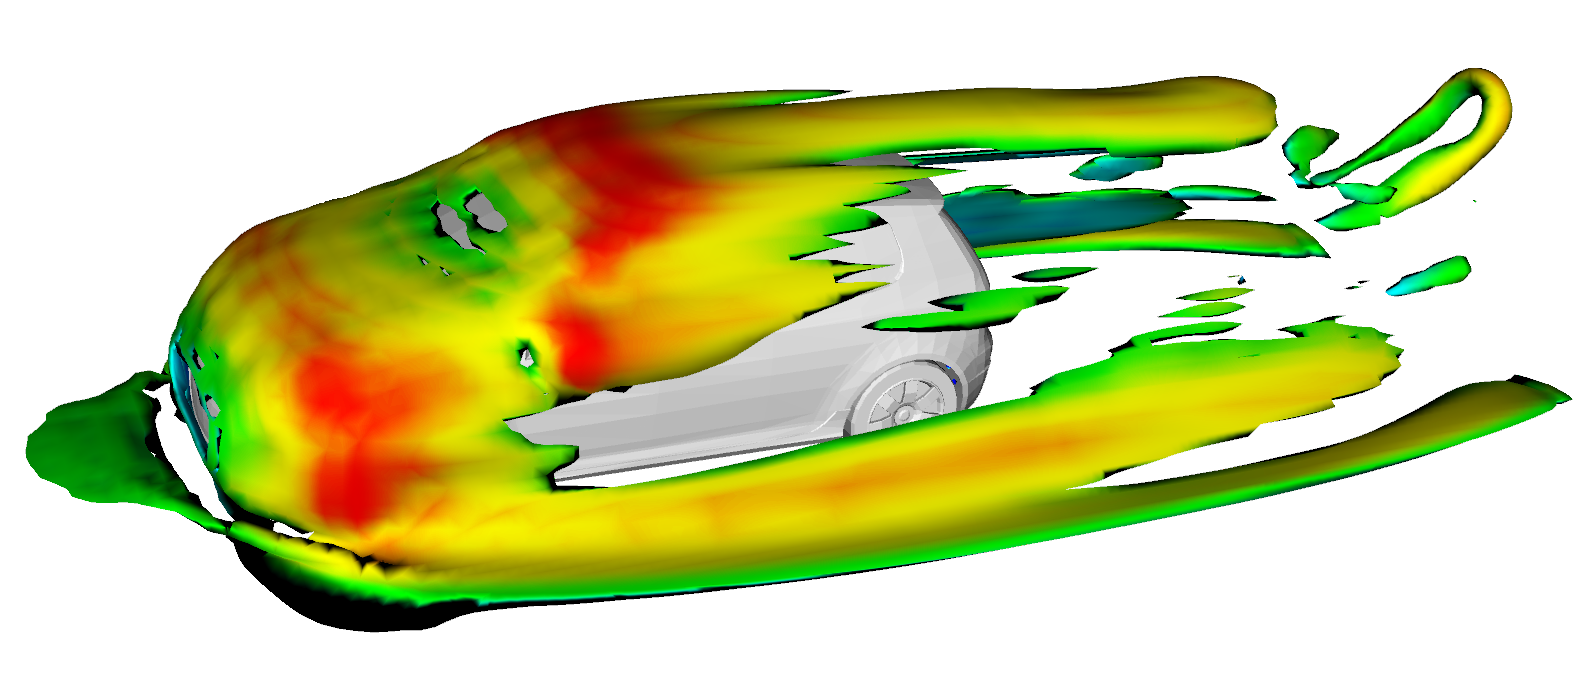
\includegraphics[width=0.8\textwidth]{img/kap1/gitSimu}
	\caption{Cooles Bild in Farbe}
	\label{fig:bild}
\end{figure} 


\section{Section mit Abkürzung}
So wird eine Akürzung benutzt \ac{ABC}

\section{Section mit Listing}
\begin{lstlisting}[caption = SomeClass., label=cs:someClass]
class SomeClass : public SomeClass{
	private:
	string variable;
	
	public:
	virtual void someMethode(){
		//...
	}
}
\end{lstlisting}

\section{Section mit Formel}
\begin{equation}
T^{s} = s + pN.
\formelentry{Problemlösezeit seriell bei schwacher Skalierung}
\label{eq:seriellSchwachSkal}
\end{equation}
